% Options for packages loaded elsewhere
\PassOptionsToPackage{unicode}{hyperref}
\PassOptionsToPackage{hyphens}{url}
%
\documentclass[
]{article}
\usepackage{amsmath,amssymb}
\usepackage{iftex}
\ifPDFTeX
  \usepackage[T1]{fontenc}
  \usepackage[utf8]{inputenc}
  \usepackage{textcomp} % provide euro and other symbols
\else % if luatex or xetex
  \usepackage{unicode-math} % this also loads fontspec
  \defaultfontfeatures{Scale=MatchLowercase}
  \defaultfontfeatures[\rmfamily]{Ligatures=TeX,Scale=1}
\fi
\usepackage{lmodern}
\ifPDFTeX\else
  % xetex/luatex font selection
\fi
% Use upquote if available, for straight quotes in verbatim environments
\IfFileExists{upquote.sty}{\usepackage{upquote}}{}
\IfFileExists{microtype.sty}{% use microtype if available
  \usepackage[]{microtype}
  \UseMicrotypeSet[protrusion]{basicmath} % disable protrusion for tt fonts
}{}
\makeatletter
\@ifundefined{KOMAClassName}{% if non-KOMA class
  \IfFileExists{parskip.sty}{%
    \usepackage{parskip}
  }{% else
    \setlength{\parindent}{0pt}
    \setlength{\parskip}{6pt plus 2pt minus 1pt}}
}{% if KOMA class
  \KOMAoptions{parskip=half}}
\makeatother
\usepackage{xcolor}
\usepackage[margin=1in]{geometry}
\usepackage{color}
\usepackage{fancyvrb}
\newcommand{\VerbBar}{|}
\newcommand{\VERB}{\Verb[commandchars=\\\{\}]}
\DefineVerbatimEnvironment{Highlighting}{Verbatim}{commandchars=\\\{\}}
% Add ',fontsize=\small' for more characters per line
\usepackage{framed}
\definecolor{shadecolor}{RGB}{248,248,248}
\newenvironment{Shaded}{\begin{snugshade}}{\end{snugshade}}
\newcommand{\AlertTok}[1]{\textcolor[rgb]{0.94,0.16,0.16}{#1}}
\newcommand{\AnnotationTok}[1]{\textcolor[rgb]{0.56,0.35,0.01}{\textbf{\textit{#1}}}}
\newcommand{\AttributeTok}[1]{\textcolor[rgb]{0.13,0.29,0.53}{#1}}
\newcommand{\BaseNTok}[1]{\textcolor[rgb]{0.00,0.00,0.81}{#1}}
\newcommand{\BuiltInTok}[1]{#1}
\newcommand{\CharTok}[1]{\textcolor[rgb]{0.31,0.60,0.02}{#1}}
\newcommand{\CommentTok}[1]{\textcolor[rgb]{0.56,0.35,0.01}{\textit{#1}}}
\newcommand{\CommentVarTok}[1]{\textcolor[rgb]{0.56,0.35,0.01}{\textbf{\textit{#1}}}}
\newcommand{\ConstantTok}[1]{\textcolor[rgb]{0.56,0.35,0.01}{#1}}
\newcommand{\ControlFlowTok}[1]{\textcolor[rgb]{0.13,0.29,0.53}{\textbf{#1}}}
\newcommand{\DataTypeTok}[1]{\textcolor[rgb]{0.13,0.29,0.53}{#1}}
\newcommand{\DecValTok}[1]{\textcolor[rgb]{0.00,0.00,0.81}{#1}}
\newcommand{\DocumentationTok}[1]{\textcolor[rgb]{0.56,0.35,0.01}{\textbf{\textit{#1}}}}
\newcommand{\ErrorTok}[1]{\textcolor[rgb]{0.64,0.00,0.00}{\textbf{#1}}}
\newcommand{\ExtensionTok}[1]{#1}
\newcommand{\FloatTok}[1]{\textcolor[rgb]{0.00,0.00,0.81}{#1}}
\newcommand{\FunctionTok}[1]{\textcolor[rgb]{0.13,0.29,0.53}{\textbf{#1}}}
\newcommand{\ImportTok}[1]{#1}
\newcommand{\InformationTok}[1]{\textcolor[rgb]{0.56,0.35,0.01}{\textbf{\textit{#1}}}}
\newcommand{\KeywordTok}[1]{\textcolor[rgb]{0.13,0.29,0.53}{\textbf{#1}}}
\newcommand{\NormalTok}[1]{#1}
\newcommand{\OperatorTok}[1]{\textcolor[rgb]{0.81,0.36,0.00}{\textbf{#1}}}
\newcommand{\OtherTok}[1]{\textcolor[rgb]{0.56,0.35,0.01}{#1}}
\newcommand{\PreprocessorTok}[1]{\textcolor[rgb]{0.56,0.35,0.01}{\textit{#1}}}
\newcommand{\RegionMarkerTok}[1]{#1}
\newcommand{\SpecialCharTok}[1]{\textcolor[rgb]{0.81,0.36,0.00}{\textbf{#1}}}
\newcommand{\SpecialStringTok}[1]{\textcolor[rgb]{0.31,0.60,0.02}{#1}}
\newcommand{\StringTok}[1]{\textcolor[rgb]{0.31,0.60,0.02}{#1}}
\newcommand{\VariableTok}[1]{\textcolor[rgb]{0.00,0.00,0.00}{#1}}
\newcommand{\VerbatimStringTok}[1]{\textcolor[rgb]{0.31,0.60,0.02}{#1}}
\newcommand{\WarningTok}[1]{\textcolor[rgb]{0.56,0.35,0.01}{\textbf{\textit{#1}}}}
\usepackage{graphicx}
\makeatletter
\def\maxwidth{\ifdim\Gin@nat@width>\linewidth\linewidth\else\Gin@nat@width\fi}
\def\maxheight{\ifdim\Gin@nat@height>\textheight\textheight\else\Gin@nat@height\fi}
\makeatother
% Scale images if necessary, so that they will not overflow the page
% margins by default, and it is still possible to overwrite the defaults
% using explicit options in \includegraphics[width, height, ...]{}
\setkeys{Gin}{width=\maxwidth,height=\maxheight,keepaspectratio}
% Set default figure placement to htbp
\makeatletter
\def\fps@figure{htbp}
\makeatother
\setlength{\emergencystretch}{3em} % prevent overfull lines
\providecommand{\tightlist}{%
  \setlength{\itemsep}{0pt}\setlength{\parskip}{0pt}}
\setcounter{secnumdepth}{-\maxdimen} % remove section numbering
\usepackage{booktabs}
\usepackage{longtable}
\usepackage{array}
\usepackage{multirow}
\usepackage{wrapfig}
\usepackage{float}
\usepackage{colortbl}
\usepackage{pdflscape}
\usepackage{tabu}
\usepackage{threeparttable}
\usepackage{threeparttablex}
\usepackage[normalem]{ulem}
\usepackage{makecell}
\usepackage{xcolor}
\ifLuaTeX
  \usepackage{selnolig}  % disable illegal ligatures
\fi
\IfFileExists{bookmark.sty}{\usepackage{bookmark}}{\usepackage{hyperref}}
\IfFileExists{xurl.sty}{\usepackage{xurl}}{} % add URL line breaks if available
\urlstyle{same}
\hypersetup{
  pdftitle={R Code},
  hidelinks,
  pdfcreator={LaTeX via pandoc}}

\title{R Code}
\author{}
\date{\vspace{-2.5em}2023-10-02}

\begin{document}
\maketitle

\hypertarget{r-markdown}{%
\subsection{R Markdown}\label{r-markdown}}

This is an R Markdown document. Markdown is a simple formatting syntax
for authoring HTML, PDF, and MS Word documents. For more details on
using R Markdown see \url{http://rmarkdown.rstudio.com}.

When you click the \textbf{Knit} button a document will be generated
that includes both content as well as the output of any embedded R code
chunks within the document. You can embed an R code chunk like this:

\begin{Shaded}
\begin{Highlighting}[]
\CommentTok{\#Load libraries and packages used for the EDA}
\FunctionTok{summary}\NormalTok{(cars)}
\end{Highlighting}
\end{Shaded}

\begin{verbatim}
##      speed           dist       
##  Min.   : 4.0   Min.   :  2.00  
##  1st Qu.:12.0   1st Qu.: 26.00  
##  Median :15.0   Median : 36.00  
##  Mean   :15.4   Mean   : 42.98  
##  3rd Qu.:19.0   3rd Qu.: 56.00  
##  Max.   :25.0   Max.   :120.00
\end{verbatim}

\begin{Shaded}
\begin{Highlighting}[]
\FunctionTok{library}\NormalTok{(tidyverse)}
\end{Highlighting}
\end{Shaded}

\begin{verbatim}
## Warning: package 'tidyverse' was built under R version 4.2.3
\end{verbatim}

\begin{verbatim}
## Warning: package 'ggplot2' was built under R version 4.2.3
\end{verbatim}

\begin{verbatim}
## Warning: package 'tibble' was built under R version 4.2.3
\end{verbatim}

\begin{verbatim}
## Warning: package 'purrr' was built under R version 4.2.3
\end{verbatim}

\begin{verbatim}
## Warning: package 'dplyr' was built under R version 4.2.3
\end{verbatim}

\begin{verbatim}
## Warning: package 'lubridate' was built under R version 4.2.3
\end{verbatim}

\begin{verbatim}
## -- Attaching core tidyverse packages ------------------------ tidyverse 2.0.0 --
## v dplyr     1.1.3     v readr     2.1.4
## v forcats   1.0.0     v stringr   1.5.0
## v ggplot2   3.4.3     v tibble    3.2.1
## v lubridate 1.9.2     v tidyr     1.3.0
## v purrr     1.0.2     
## -- Conflicts ------------------------------------------ tidyverse_conflicts() --
## x dplyr::filter() masks stats::filter()
## x dplyr::lag()    masks stats::lag()
## i Use the conflicted package (<http://conflicted.r-lib.org/>) to force all conflicts to become errors
\end{verbatim}

\begin{Shaded}
\begin{Highlighting}[]
\FunctionTok{library}\NormalTok{(dplyr)}
\FunctionTok{library}\NormalTok{(kableExtra)}
\end{Highlighting}
\end{Shaded}

\begin{verbatim}
## Warning in !is.null(rmarkdown::metadata$output) && rmarkdown::metadata$output
## %in% : 'length(x) = 2 > 1' in coercion to 'logical(1)'
\end{verbatim}

\begin{verbatim}
## 
## Attaching package: 'kableExtra'
## 
## The following object is masked from 'package:dplyr':
## 
##     group_rows
\end{verbatim}

\begin{Shaded}
\begin{Highlighting}[]
\FunctionTok{library}\NormalTok{(gtsummary)}
\end{Highlighting}
\end{Shaded}

\begin{verbatim}
## Warning: package 'gtsummary' was built under R version 4.2.3
\end{verbatim}

\begin{Shaded}
\begin{Highlighting}[]
\FunctionTok{library}\NormalTok{(ggplot2)}
\FunctionTok{library}\NormalTok{(naniar)}
\end{Highlighting}
\end{Shaded}

\begin{verbatim}
## Warning: package 'naniar' was built under R version 4.2.3
\end{verbatim}

\hypertarget{including-plots}{%
\subsection{Including Plots}\label{including-plots}}

You can also embed plots, for example:

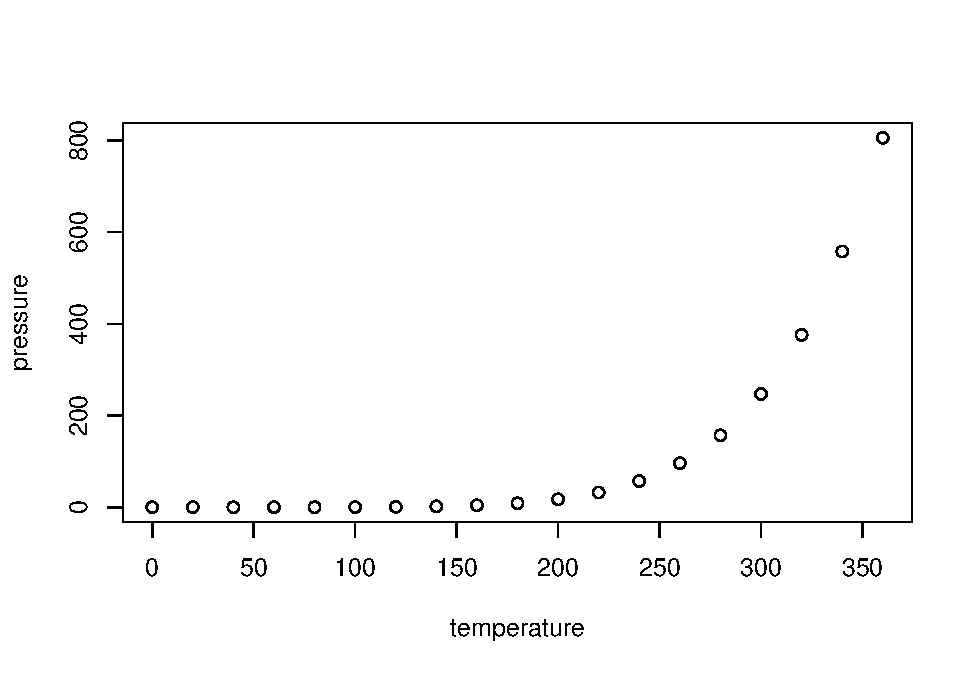
\includegraphics{Project-1-PHP-2550_files/figure-latex/pressure-1.pdf}

Note that the \texttt{echo\ =\ FALSE} parameter was added to the code
chunk to prevent printing of the R code that generated the plot.

\#Ask about the 0 in num cigs and see if they are supposed to all of the
NAs be 0

\begin{Shaded}
\begin{Highlighting}[]
\NormalTok{new\_df[,}\FunctionTok{c}\NormalTok{(}\DecValTok{22}\SpecialCharTok{:}\DecValTok{28}\NormalTok{)]}\OtherTok{\textless{}{-}}\FunctionTok{lapply}\NormalTok{(new\_df[,}\FunctionTok{c}\NormalTok{ (}\DecValTok{22}\SpecialCharTok{:}\DecValTok{28}\NormalTok{)],}\ControlFlowTok{function}\NormalTok{(x) }\FunctionTok{ifelse}\NormalTok{(x}\SpecialCharTok{==}\StringTok{""}\NormalTok{,}\ConstantTok{NA}\NormalTok{,x))}
\CommentTok{\#new\_df[c,22:28] \textless{}{-} lapply(new\_df[,22:28], function(x) ifelse(x == "1=Yes", 1, x))}
\CommentTok{\#new\_df[c,22:28] \textless{}{-} lapply(new\_df[,22:28], function(x) ifelse(x == "2=No", 0, x))}

\CommentTok{\#Factor character variables in dataset}
\NormalTok{new\_df}\OtherTok{\textless{}{-}}\NormalTok{new\_df }\SpecialCharTok{\%\textgreater{}\%}
  \FunctionTok{mutate\_if}\NormalTok{(is.character,factor)}


\NormalTok{new\_df[}\DecValTok{1}\NormalTok{,}\DecValTok{21}\NormalTok{]}\OtherTok{\textless{}{-}}\DecValTok{2}
\NormalTok{new\_df[}\DecValTok{47}\NormalTok{,}\DecValTok{21}\NormalTok{]}\OtherTok{\textless{}{-}}\DecValTok{0}
\NormalTok{new\_df[}\DecValTok{26}\NormalTok{,}\DecValTok{21}\NormalTok{]}\OtherTok{\textless{}{-}}\ConstantTok{NA}


\CommentTok{\# Assuming your data frame is named \textquotesingle{}df\textquotesingle{} and you want to remove the row at index \textquotesingle{}row\_to\_remove\textquotesingle{}}
\NormalTok{row\_to\_remove }\OtherTok{\textless{}{-}} \DecValTok{38}  \CommentTok{\# Replace with the index of the row you want to remove}
\NormalTok{new\_df }\OtherTok{\textless{}{-}}\NormalTok{ new\_df[}\SpecialCharTok{{-}}\NormalTok{row\_to\_remove, ]}


\CommentTok{\#head(new\_df)}
\end{Highlighting}
\end{Shaded}

\begin{Shaded}
\begin{Highlighting}[]
\CommentTok{\#Find average composite score of follow up}
\NormalTok{new\_df}\SpecialCharTok{$}\NormalTok{avg\_smoke\_follow}\OtherTok{\textless{}{-}}\NormalTok{((}\FunctionTok{rowSums}\NormalTok{(new\_df[,}\FunctionTok{c}\NormalTok{(}\StringTok{"smoke\_exposure\_6mo"}\NormalTok{,}\StringTok{"smoke\_exposure\_12mo"}\NormalTok{)] }\SpecialCharTok{==}\DecValTok{1}\NormalTok{,}
                                    \AttributeTok{na.rm=}\NormalTok{T))}\SpecialCharTok{/}\DecValTok{2}
                           \SpecialCharTok{+}\NormalTok{(}\FunctionTok{rowSums}\NormalTok{(new\_df[,}\FunctionTok{c}\NormalTok{(}\StringTok{"smoke\_exposure\_2yr"}\NormalTok{,}\StringTok{"smoke\_exposure\_3yr"}\NormalTok{,}
                                               \StringTok{"smoke\_exposure\_4yr"}\NormalTok{,}\StringTok{"smoke\_exposure\_5yr"}\NormalTok{)] }\SpecialCharTok{==}\DecValTok{1}\NormalTok{,}
                                           \AttributeTok{na.rm=}\NormalTok{ T)))}\SpecialCharTok{/}\DecValTok{5}
                                  
\NormalTok{new\_df}\SpecialCharTok{$}\NormalTok{cum\_smoke\_pp}\OtherTok{\textless{}{-}}\NormalTok{(}\FunctionTok{rowSums}\NormalTok{(new\_df[,}\FunctionTok{c}\NormalTok{(}\StringTok{"mom\_smoke\_pp12wk"}\NormalTok{,}\StringTok{"mom\_smoke\_pp6mo"}\NormalTok{)]}\SpecialCharTok{==}\StringTok{"1=Yes"}\NormalTok{,}
  
                              
                                                         \AttributeTok{na.rm=}\NormalTok{T))}

\CommentTok{\#Find cumulative score of SDP}
\NormalTok{new\_df}\SpecialCharTok{$}\NormalTok{cum\_smoke\_preg}\OtherTok{\textless{}{-}}\FunctionTok{rowSums}\NormalTok{(new\_df[,}\FunctionTok{c}\NormalTok{(}\StringTok{"mom\_smoke\_16wk"}\NormalTok{,}
                            \StringTok{"mom\_smoke\_22wk"}\NormalTok{, }
                            \StringTok{"mom\_smoke\_32wk"}\NormalTok{)] }\SpecialCharTok{==} \StringTok{"1=Yes"}\NormalTok{,}
                    \AttributeTok{na.rm =}\NormalTok{ T)}
\end{Highlighting}
\end{Shaded}

\begin{Shaded}
\begin{Highlighting}[]
\CommentTok{\#Summarize baseline characteristics }
\end{Highlighting}
\end{Shaded}

\begin{Shaded}
\begin{Highlighting}[]
\CommentTok{\#Look at missing Data for each variable in study }
\NormalTok{overall\_missing}\OtherTok{\textless{}{-}}\FunctionTok{miss\_var\_summary}\NormalTok{(new\_df)}
\NormalTok{overall\_missing}
\end{Highlighting}
\end{Shaded}

\begin{verbatim}
## # A tibble: 81 x 3
##    variable                   n_miss pct_miss
##    <chr>                       <int>    <dbl>
##  1 num_cigs_30                    47     97.9
##  2 num_e_cigs_30                  46     95.8
##  3 num_mj_30                      45     93.8
##  4 num_alc_30                     44     91.7
##  5 mom_smoke_pp1                  38     79.2
##  6 childasd                       28     58.3
##  7 mom_smoke_pp2                  19     39.6
##  8 pmq_parental_control           15     31.2
##  9 ppmq_parental_solicitation     14     29.2
## 10 bpm_int                        13     27.1
## # i 71 more rows
\end{verbatim}

\begin{Shaded}
\begin{Highlighting}[]
\CommentTok{\#Look at missing data for each parent }
\NormalTok{pct\_na\_r }\OtherTok{\textless{}{-}} \FunctionTok{rowSums}\NormalTok{(}\FunctionTok{is.na}\NormalTok{(new\_df)) }\SpecialCharTok{/} \FunctionTok{ncol}\NormalTok{(new\_df) }\SpecialCharTok{*} \DecValTok{100}
\NormalTok{row\_na }\OtherTok{\textless{}{-}} \FunctionTok{data.frame}\NormalTok{(}\AttributeTok{parent\_id =}\NormalTok{ new\_df}\SpecialCharTok{$}\NormalTok{parent\_id, }\AttributeTok{pct\_na =}\NormalTok{ pct\_na\_r)}
\NormalTok{row\_na }\OtherTok{\textless{}{-}}\NormalTok{ row\_na[row\_na}\SpecialCharTok{$}\NormalTok{pct\_na }\SpecialCharTok{\textgreater{}} \DecValTok{40}\NormalTok{,] }\CommentTok{\# participants with greater than 40\% missing}
\FunctionTok{print}\NormalTok{(row\_na) }
\end{Highlighting}
\end{Shaded}

\begin{verbatim}
##    parent_id   pct_na
## 5      50502 66.66667
## 12     51202 64.19753
## 16     51602 69.13580
## 22     52302 64.19753
## 34     53502 43.20988
## 43     54402 69.13580
## 45     54602 69.13580
## 46     54702 65.43210
\end{verbatim}

\begin{Shaded}
\begin{Highlighting}[]
\CommentTok{\#missingness plot with percentages for pre and postpartum }

\NormalTok{post\_pre\_plot}\OtherTok{\textless{}{-}}\FunctionTok{gg\_miss\_var}\NormalTok{(}\AttributeTok{show\_pct =} \ConstantTok{TRUE}\NormalTok{, new\_df }\SpecialCharTok{\%\textgreater{}\%}
             \FunctionTok{select}\NormalTok{(mom\_smoke\_16wk}\SpecialCharTok{:}\NormalTok{mom\_smoke\_pp6mo))}
\NormalTok{post\_pre\_plot}
\end{Highlighting}
\end{Shaded}

\includegraphics{Project-1-PHP-2550_files/figure-latex/unnamed-chunk-4-1.pdf}

\begin{Shaded}
\begin{Highlighting}[]
\CommentTok{\#Missingness plot with percentages for follow up}

\NormalTok{follow\_up\_na\_plot}\OtherTok{\textless{}{-}}\FunctionTok{gg\_miss\_var}\NormalTok{(}\AttributeTok{show\_pct =} \ConstantTok{TRUE}\NormalTok{, new\_df }\SpecialCharTok{\%\textgreater{}\%}
             \FunctionTok{select}\NormalTok{(smoke\_exposure\_6mo}\SpecialCharTok{:}\NormalTok{smoke\_exposure\_5yr))}
\NormalTok{follow\_up\_na\_plot}
\end{Highlighting}
\end{Shaded}

\includegraphics{Project-1-PHP-2550_files/figure-latex/unnamed-chunk-4-2.pdf}

\begin{Shaded}
\begin{Highlighting}[]
\CommentTok{\#Also keep on the lookout for the person who smoked 45,000 cigarettes a day they might need to be removed as well}
\end{Highlighting}
\end{Shaded}

AIM 1: Examine effects of SDP/ETS on adolescent self-regulation,
substance use, and externalizing.

\begin{Shaded}
\begin{Highlighting}[]
\CommentTok{\#Look at self regulation variables which include bpm\_att,bpm\_ext,bpm\_int,erq\_cog,erq\_exp}


\CommentTok{\#summarize 6 months (together) in comparison to followups in the }
\CommentTok{\#eda for univaritates summary for plots}


\NormalTok{new\_df}\SpecialCharTok{$}\NormalTok{mom\_smoke\_32wk}\OtherTok{\textless{}{-}} \FunctionTok{ifelse}\NormalTok{(new\_df}\SpecialCharTok{$}\NormalTok{mom\_smoke\_16wk }\SpecialCharTok{==} \StringTok{"1=Yes"} \SpecialCharTok{\&} 
\NormalTok{                                 new\_df}\SpecialCharTok{$}\NormalTok{mom\_smoke\_22wk }\SpecialCharTok{==} \StringTok{"1=Yes"}\NormalTok{,}
                  \StringTok{"1=Yes"}\NormalTok{, }\FunctionTok{as.character}\NormalTok{(new\_df}\SpecialCharTok{$}\NormalTok{mom\_smoke\_32wk) )}

\NormalTok{new\_df}\SpecialCharTok{$}\NormalTok{mom\_smoke\_pp1}\OtherTok{\textless{}{-}} \FunctionTok{ifelse}\NormalTok{(new\_df}\SpecialCharTok{$}\NormalTok{mom\_smoke\_22wk }\SpecialCharTok{==} \StringTok{"1=Yes"} \SpecialCharTok{\&} 
\NormalTok{                               new\_df}\SpecialCharTok{$}\NormalTok{mom\_smoke\_32wk }\SpecialCharTok{==} \StringTok{"1=Yes"} \SpecialCharTok{\&}
\NormalTok{                               new\_df}\SpecialCharTok{$}\NormalTok{mom\_smoke\_pp2 }\SpecialCharTok{==} \StringTok{"1=Yes"}\NormalTok{,}
                  \StringTok{"1=Yes"}\NormalTok{, }\FunctionTok{as.character}\NormalTok{(new\_df}\SpecialCharTok{$}\NormalTok{mom\_smoke\_pp1)) }
\end{Highlighting}
\end{Shaded}

\begin{Shaded}
\begin{Highlighting}[]
\CommentTok{\#look at substance use variables include: cig\_ever,e\_cig\_ever,alc\_ever,mj\_ever}
\NormalTok{tbl\_cig\_child}\OtherTok{\textless{}{-}}\NormalTok{new\_df}\SpecialCharTok{\%\textgreater{}\%}
  \FunctionTok{count}\NormalTok{(cig\_ever)}
\NormalTok{tbl\_ecig\_child}\OtherTok{\textless{}{-}}\NormalTok{new\_df}\SpecialCharTok{\%\textgreater{}\%}
  \FunctionTok{count}\NormalTok{(e\_cig\_ever)}
\NormalTok{tbl\_alc\_child}\OtherTok{\textless{}{-}}\NormalTok{new\_df}\SpecialCharTok{\%\textgreater{}\%}
  \FunctionTok{count}\NormalTok{(alc\_ever)}
\NormalTok{tbl\_mj\_child}\OtherTok{\textless{}{-}}\NormalTok{new\_df}\SpecialCharTok{\%\textgreater{}\%}
  \FunctionTok{count}\NormalTok{(mj\_ever)}
\NormalTok{all\_sub\_counts}\OtherTok{\textless{}{-}}\FunctionTok{bind\_cols}\NormalTok{(tbl\_mj\_child,tbl\_alc\_child,tbl\_ecig\_child,tbl\_cig\_child)}
\end{Highlighting}
\end{Shaded}

\begin{verbatim}
## New names:
## * `n` -> `n...2`
## * `n` -> `n...4`
## * `n` -> `n...6`
## * `n` -> `n...8`
\end{verbatim}

\begin{Shaded}
\begin{Highlighting}[]
\CommentTok{\#all\_sub\_counts}

\CommentTok{\#Subset data for the number of substance use}

\CommentTok{\#Create a cumulative score of the smoking status while the mother was pregnant}
\NormalTok{new\_df}\SpecialCharTok{$}\NormalTok{mom\_smoke\_16wk}\OtherTok{\textless{}{-}}\FunctionTok{factor}\NormalTok{(new\_df}\SpecialCharTok{$}\NormalTok{mom\_smoke\_16wk)}
\NormalTok{new\_df}\SpecialCharTok{$}\NormalTok{mom\_smoke\_22wk}\OtherTok{\textless{}{-}}\FunctionTok{factor}\NormalTok{(new\_df}\SpecialCharTok{$}\NormalTok{mom\_smoke\_22wk)}
\NormalTok{new\_df}\SpecialCharTok{$}\NormalTok{mom\_smoke\_32wk}\OtherTok{\textless{}{-}}\FunctionTok{factor}\NormalTok{(new\_df}\SpecialCharTok{$}\NormalTok{mom\_smoke\_32wk)}


\CommentTok{\#For pre and post{-}partum create proportions table and evaluate the effects on if someone said yes to substances compared to each smoking status }


\CommentTok{\#fit new model using cumulative count with alcohol use }

\NormalTok{model\_cum\_smoke\_alc}\OtherTok{\textless{}{-}} \FunctionTok{glm}\NormalTok{(alc\_ever }\SpecialCharTok{\textasciitilde{}}\NormalTok{ cum\_smoke\_preg, }\AttributeTok{data =}\NormalTok{ new\_df, }\AttributeTok{family =} \FunctionTok{binomial}\NormalTok{(}\AttributeTok{link =} \StringTok{"logit"}\NormalTok{))}
\FunctionTok{summary}\NormalTok{(model\_cum\_smoke\_alc)}
\end{Highlighting}
\end{Shaded}

\begin{verbatim}
## 
## Call:
## glm(formula = alc_ever ~ cum_smoke_preg, family = binomial(link = "logit"), 
##     data = new_df)
## 
## Deviance Residuals: 
##     Min       1Q   Median       3Q      Max  
## -0.8664  -0.4383  -0.4383  -0.4383   2.1866  
## 
## Coefficients:
##                Estimate Std. Error z value Pr(>|z|)    
## (Intercept)     -2.2945     0.6563  -3.496 0.000472 ***
## cum_smoke_preg   0.5027     0.3534   1.422 0.154943    
## ---
## Signif. codes:  0 '***' 0.001 '**' 0.01 '*' 0.05 '.' 0.1 ' ' 1
## 
## (Dispersion parameter for binomial family taken to be 1)
## 
##     Null deviance: 29.012  on 35  degrees of freedom
## Residual deviance: 27.081  on 34  degrees of freedom
##   (12 observations deleted due to missingness)
## AIC: 31.081
## 
## Number of Fisher Scoring iterations: 5
\end{verbatim}

\begin{Shaded}
\begin{Highlighting}[]
\CommentTok{\#create plot showing the probability predictions }
\NormalTok{new\_cum\_data }\OtherTok{\textless{}{-}} \FunctionTok{data.frame}\NormalTok{(}\AttributeTok{cum\_smoke\_preg =}\NormalTok{ new\_df}\SpecialCharTok{$}\NormalTok{cum\_smoke\_preg)}

\CommentTok{\# Predict probabilities using the model}
\NormalTok{new\_cum\_data}\SpecialCharTok{$}\NormalTok{Predicted\_Probabilities}\OtherTok{\textless{}{-}} \FunctionTok{predict}\NormalTok{(model\_cum\_smoke\_alc, }\AttributeTok{newdata =}\NormalTok{ new\_cum\_data, }\AttributeTok{type =} \StringTok{"response"}\NormalTok{)}


\CommentTok{\# Create a plot for baseline and alcohol use predictions}
\FunctionTok{ggplot}\NormalTok{(}\AttributeTok{data =}\NormalTok{ new\_cum\_data, }\FunctionTok{aes}\NormalTok{(}\AttributeTok{x =}\NormalTok{ cum\_smoke\_preg, }\AttributeTok{y =}\NormalTok{ Predicted\_Probabilities)) }\SpecialCharTok{+}
  \FunctionTok{geom\_line}\NormalTok{() }\SpecialCharTok{+}
  \FunctionTok{labs}\NormalTok{(}
    \AttributeTok{x =} \StringTok{"Maternal Smoking Status Cumulative"}\NormalTok{,}
    \AttributeTok{y =} \StringTok{"Predicted Probabilities of Child Alcohol Use"}\NormalTok{,}
    \AttributeTok{title =} \StringTok{"Logistic Regression Predicted Probabilities"}
\NormalTok{  )}
\end{Highlighting}
\end{Shaded}

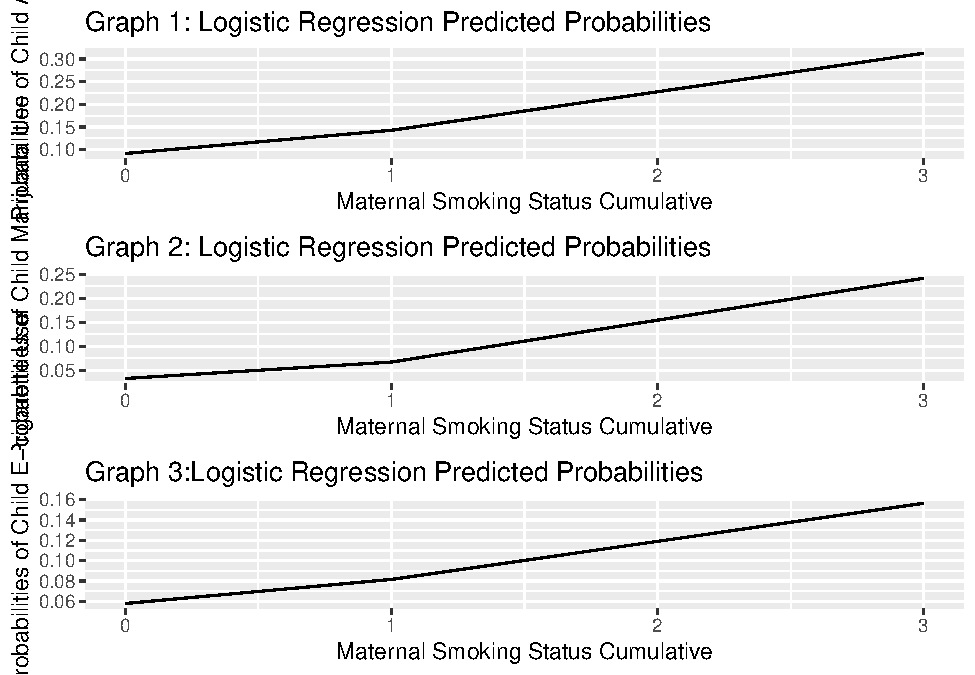
\includegraphics{Project-1-PHP-2550_files/figure-latex/unnamed-chunk-6-1.pdf}

\begin{Shaded}
\begin{Highlighting}[]
\CommentTok{\#fit new model using average of follow up scores with child\textquotesingle{}s alcohol use }

\NormalTok{model\_avg\_smoke\_alc}\OtherTok{\textless{}{-}} \FunctionTok{glm}\NormalTok{(alc\_ever }\SpecialCharTok{\textasciitilde{}}\NormalTok{ avg\_smoke\_follow, }\AttributeTok{data =}\NormalTok{ new\_df, }\AttributeTok{family =} \FunctionTok{binomial}\NormalTok{(}\AttributeTok{link =} \StringTok{"logit"}\NormalTok{))}
\FunctionTok{summary}\NormalTok{(model\_avg\_smoke\_alc)}
\end{Highlighting}
\end{Shaded}

\begin{verbatim}
## 
## Call:
## glm(formula = alc_ever ~ avg_smoke_follow, family = binomial(link = "logit"), 
##     data = new_df)
## 
## Deviance Residuals: 
##     Min       1Q   Median       3Q      Max  
## -0.5721  -0.5721  -0.5721  -0.4834   2.1124  
## 
## Coefficients:
##                  Estimate Std. Error z value Pr(>|z|)   
## (Intercept)       -1.7272     0.5616  -3.075   0.0021 **
## avg_smoke_follow  -0.3904     1.2639  -0.309   0.7574   
## ---
## Signif. codes:  0 '***' 0.001 '**' 0.01 '*' 0.05 '.' 0.1 ' ' 1
## 
## (Dispersion parameter for binomial family taken to be 1)
## 
##     Null deviance: 29.012  on 35  degrees of freedom
## Residual deviance: 28.912  on 34  degrees of freedom
##   (12 observations deleted due to missingness)
## AIC: 32.912
## 
## Number of Fisher Scoring iterations: 4
\end{verbatim}

\begin{Shaded}
\begin{Highlighting}[]
\CommentTok{\#create plot showing the probability predictions }
\NormalTok{new\_avg\_follow}\OtherTok{\textless{}{-}} \FunctionTok{data.frame}\NormalTok{(}\AttributeTok{avg\_smoke\_follow =}\NormalTok{ new\_df}\SpecialCharTok{$}\NormalTok{avg\_smoke\_follow)}

\CommentTok{\# Predict probabilities using the model}
\NormalTok{new\_avg\_follow}\SpecialCharTok{$}\NormalTok{Predicted\_Prob\_avg}\OtherTok{\textless{}{-}} \FunctionTok{predict}\NormalTok{(model\_avg\_smoke\_alc, }\AttributeTok{newdata =}\NormalTok{ new\_avg\_follow, }\AttributeTok{type =} \StringTok{"response"}\NormalTok{)}


\CommentTok{\# Create a plot for baseline and alcohol use predictions}
\FunctionTok{ggplot}\NormalTok{(}\AttributeTok{data =}\NormalTok{ new\_avg\_follow, }\FunctionTok{aes}\NormalTok{(}\AttributeTok{x =}\NormalTok{ avg\_smoke\_follow, }\AttributeTok{y =}\NormalTok{ Predicted\_Prob\_avg)) }\SpecialCharTok{+}
  \FunctionTok{geom\_line}\NormalTok{() }\SpecialCharTok{+}
  \FunctionTok{labs}\NormalTok{(}
    \AttributeTok{x =} \StringTok{"Maternal Smoking Status Follow up Average"}\NormalTok{,}
    \AttributeTok{y =} \StringTok{"Predicted Probabilities of Child Alcohol Use"}\NormalTok{,}
    \AttributeTok{title =} \StringTok{"Logistic Regression Predicted Probabilities"}
\NormalTok{  )}
\end{Highlighting}
\end{Shaded}

\includegraphics{Project-1-PHP-2550_files/figure-latex/unnamed-chunk-8-1.pdf}

\begin{Shaded}
\begin{Highlighting}[]
\CommentTok{\#some of the variables are correlates so it would be useful to group them and since theyre correlatesd}
\CommentTok{\#using a model would give bias }
\CommentTok{\#fit new model using cumulative count with alcohol use }

\NormalTok{model\_cum\_smoke\_mj}\OtherTok{\textless{}{-}} \FunctionTok{glm}\NormalTok{(mj\_ever }\SpecialCharTok{\textasciitilde{}}\NormalTok{ cum\_smoke\_preg, }\AttributeTok{data =}\NormalTok{ new\_df, }\AttributeTok{family =} \FunctionTok{binomial}\NormalTok{(}\AttributeTok{link =} \StringTok{"logit"}\NormalTok{))}
\FunctionTok{summary}\NormalTok{(model\_cum\_smoke\_mj)}
\end{Highlighting}
\end{Shaded}

\begin{verbatim}
## 
## Call:
## glm(formula = mj_ever ~ cum_smoke_preg, family = binomial(link = "logit"), 
##     data = new_df)
## 
## Deviance Residuals: 
##     Min       1Q   Median       3Q      Max  
## -0.7437  -0.2602  -0.2602  -0.2602   2.6088  
## 
## Coefficients:
##                Estimate Std. Error z value Pr(>|z|)   
## (Intercept)     -3.3690     1.0431  -3.230  0.00124 **
## cum_smoke_preg   0.7417     0.4501   1.648  0.09937 . 
## ---
## Signif. codes:  0 '***' 0.001 '**' 0.01 '*' 0.05 '.' 0.1 ' ' 1
## 
## (Dispersion parameter for binomial family taken to be 1)
## 
##     Null deviance: 20.824  on 36  degrees of freedom
## Residual deviance: 17.917  on 35  degrees of freedom
##   (11 observations deleted due to missingness)
## AIC: 21.917
## 
## Number of Fisher Scoring iterations: 6
\end{verbatim}

\begin{Shaded}
\begin{Highlighting}[]
\CommentTok{\#create plot showing the probability predictions }
\NormalTok{new\_cum\_data\_mj}\OtherTok{\textless{}{-}} \FunctionTok{data.frame}\NormalTok{(}\AttributeTok{cum\_smoke\_preg =}\NormalTok{ new\_df}\SpecialCharTok{$}\NormalTok{cum\_smoke\_preg)}

\CommentTok{\# Predict probabilities using the model}
\NormalTok{new\_cum\_data\_mj}\SpecialCharTok{$}\NormalTok{Predicted\_Probabilities}\OtherTok{\textless{}{-}} \FunctionTok{predict}\NormalTok{(model\_cum\_smoke\_mj, }\AttributeTok{newdata =}\NormalTok{ new\_cum\_data\_mj, }\AttributeTok{type =} \StringTok{"response"}\NormalTok{)}


\CommentTok{\# Create a plot for baseline and alcohol use predictions}
\FunctionTok{ggplot}\NormalTok{(}\AttributeTok{data =}\NormalTok{ new\_cum\_data\_mj, }\FunctionTok{aes}\NormalTok{(}\AttributeTok{x =}\NormalTok{ cum\_smoke\_preg, }\AttributeTok{y =}\NormalTok{ Predicted\_Probabilities)) }\SpecialCharTok{+}
  \FunctionTok{geom\_line}\NormalTok{() }\SpecialCharTok{+}
  \FunctionTok{labs}\NormalTok{(}
    \AttributeTok{x =} \StringTok{"Maternal Smoking Status Cumulative"}\NormalTok{,}
    \AttributeTok{y =} \StringTok{"Predicted Probabilities of Child Marijuana Use"}\NormalTok{,}
    \AttributeTok{title =} \StringTok{"Logistic Regression Predicted Probabilities"}
\NormalTok{  )}
\end{Highlighting}
\end{Shaded}

\includegraphics{Project-1-PHP-2550_files/figure-latex/unnamed-chunk-9-1.pdf}

\begin{Shaded}
\begin{Highlighting}[]
\NormalTok{model\_cum\_smoke\_ecig}\OtherTok{\textless{}{-}} \FunctionTok{glm}\NormalTok{(e\_cig\_ever }\SpecialCharTok{\textasciitilde{}}\NormalTok{ cum\_smoke\_preg, }\AttributeTok{data =}\NormalTok{ new\_df, }\AttributeTok{family =} \FunctionTok{binomial}\NormalTok{(}\AttributeTok{link =} \StringTok{"logit"}\NormalTok{))}
\FunctionTok{summary}\NormalTok{(model\_cum\_smoke\_ecig)}
\end{Highlighting}
\end{Shaded}

\begin{verbatim}
## 
## Call:
## glm(formula = e_cig_ever ~ cum_smoke_preg, family = binomial(link = "logit"), 
##     data = new_df)
## 
## Deviance Residuals: 
##     Min       1Q   Median       3Q      Max  
## -0.5834  -0.3452  -0.3452  -0.3452   2.3876  
## 
## Coefficients:
##                Estimate Std. Error z value Pr(>|z|)    
## (Intercept)     -2.7906     0.8126  -3.434 0.000595 ***
## cum_smoke_preg   0.3687     0.4279   0.862 0.388950    
## ---
## Signif. codes:  0 '***' 0.001 '**' 0.01 '*' 0.05 '.' 0.1 ' ' 1
## 
## (Dispersion parameter for binomial family taken to be 1)
## 
##     Null deviance: 20.824  on 36  degrees of freedom
## Residual deviance: 20.125  on 35  degrees of freedom
##   (11 observations deleted due to missingness)
## AIC: 24.125
## 
## Number of Fisher Scoring iterations: 5
\end{verbatim}

\begin{Shaded}
\begin{Highlighting}[]
\CommentTok{\#create plot showing the probability predictions }
\NormalTok{new\_cum\_data\_ecig}\OtherTok{\textless{}{-}} \FunctionTok{data.frame}\NormalTok{(}\AttributeTok{cum\_smoke\_preg =}\NormalTok{ new\_df}\SpecialCharTok{$}\NormalTok{cum\_smoke\_preg)}

\CommentTok{\# Predict probabilities using the model}
\NormalTok{new\_cum\_data\_ecig}\SpecialCharTok{$}\NormalTok{Predicted\_Probabilities}\OtherTok{\textless{}{-}} \FunctionTok{predict}\NormalTok{(model\_cum\_smoke\_ecig, }\AttributeTok{newdata =}\NormalTok{ new\_cum\_data\_ecig, }\AttributeTok{type =} \StringTok{"response"}\NormalTok{)}


\CommentTok{\# Create a plot for baseline and alcohol use predictions}
\FunctionTok{ggplot}\NormalTok{(}\AttributeTok{data =}\NormalTok{ new\_cum\_data\_ecig, }\FunctionTok{aes}\NormalTok{(}\AttributeTok{x =}\NormalTok{ cum\_smoke\_preg, }\AttributeTok{y =}\NormalTok{ Predicted\_Probabilities)) }\SpecialCharTok{+}
  \FunctionTok{geom\_line}\NormalTok{() }\SpecialCharTok{+}
  \FunctionTok{labs}\NormalTok{(}
    \AttributeTok{x =} \StringTok{"Maternal Smoking Status Cumulative"}\NormalTok{,}
    \AttributeTok{y =} \StringTok{"Predicted Probabilities of Child E{-}cigarette Use"}\NormalTok{,}
    \AttributeTok{title =} \StringTok{"Logistic Regression Predicted Probabilities"}
\NormalTok{  )}
\end{Highlighting}
\end{Shaded}

\includegraphics{Project-1-PHP-2550_files/figure-latex/unnamed-chunk-10-1.pdf}

\begin{Shaded}
\begin{Highlighting}[]
\NormalTok{model\_cum\_smoke\_cig}\OtherTok{\textless{}{-}} \FunctionTok{glm}\NormalTok{(cig\_ever }\SpecialCharTok{\textasciitilde{}}\NormalTok{ cum\_smoke\_preg, }\AttributeTok{data =}\NormalTok{ new\_df, }\AttributeTok{family =} \FunctionTok{binomial}\NormalTok{(}\AttributeTok{link =} \StringTok{"logit"}\NormalTok{))}
\FunctionTok{summary}\NormalTok{(model\_cum\_smoke\_cig)}
\end{Highlighting}
\end{Shaded}

\begin{verbatim}
## 
## Call:
## glm(formula = cig_ever ~ cum_smoke_preg, family = binomial(link = "logit"), 
##     data = new_df)
## 
## Deviance Residuals: 
##      Min        1Q    Median        3Q       Max  
## -0.51678  -0.00007   0.00000   0.00000   2.03933  
## 
## Coefficients:
##                 Estimate Std. Error z value Pr(>|z|)
## (Intercept)      -28.637  10143.766  -0.003    0.998
## cum_smoke_preg     8.897   3381.255   0.003    0.998
## 
## (Dispersion parameter for binomial family taken to be 1)
## 
##     Null deviance: 9.1946  on 36  degrees of freedom
## Residual deviance: 6.0283  on 35  degrees of freedom
##   (11 observations deleted due to missingness)
## AIC: 10.028
## 
## Number of Fisher Scoring iterations: 21
\end{verbatim}

\begin{Shaded}
\begin{Highlighting}[]
\CommentTok{\#create plot showing the probability predictions }
\NormalTok{new\_cum\_data\_cig}\OtherTok{\textless{}{-}} \FunctionTok{data.frame}\NormalTok{(}\AttributeTok{cum\_smoke\_preg =}\NormalTok{ new\_df}\SpecialCharTok{$}\NormalTok{cum\_smoke\_preg)}

\CommentTok{\# Predict probabilities using the model}
\NormalTok{new\_cum\_data\_cig}\SpecialCharTok{$}\NormalTok{Predicted\_Probabilities}\OtherTok{\textless{}{-}} \FunctionTok{predict}\NormalTok{(model\_cum\_smoke\_cig, }\AttributeTok{newdata =}\NormalTok{ new\_cum\_data\_cig, }\AttributeTok{type =} \StringTok{"response"}\NormalTok{)}


\CommentTok{\# Create a plot for baseline and alcohol use predictions}
\FunctionTok{ggplot}\NormalTok{(}\AttributeTok{data =}\NormalTok{ new\_cum\_data\_cig, }\FunctionTok{aes}\NormalTok{(}\AttributeTok{x =}\NormalTok{ cum\_smoke\_preg, }\AttributeTok{y =}\NormalTok{ Predicted\_Probabilities)) }\SpecialCharTok{+}
  \FunctionTok{geom\_line}\NormalTok{() }\SpecialCharTok{+}
  \FunctionTok{labs}\NormalTok{(}
    \AttributeTok{x =} \StringTok{"Maternal Smoking Status Cumulative"}\NormalTok{,}
    \AttributeTok{y =} \StringTok{"Predicted Probabilities of Child cigarette Use"}\NormalTok{,}
    \AttributeTok{title =} \StringTok{"Logistic Regression Predicted Probabilities"}
\NormalTok{)}
\end{Highlighting}
\end{Shaded}

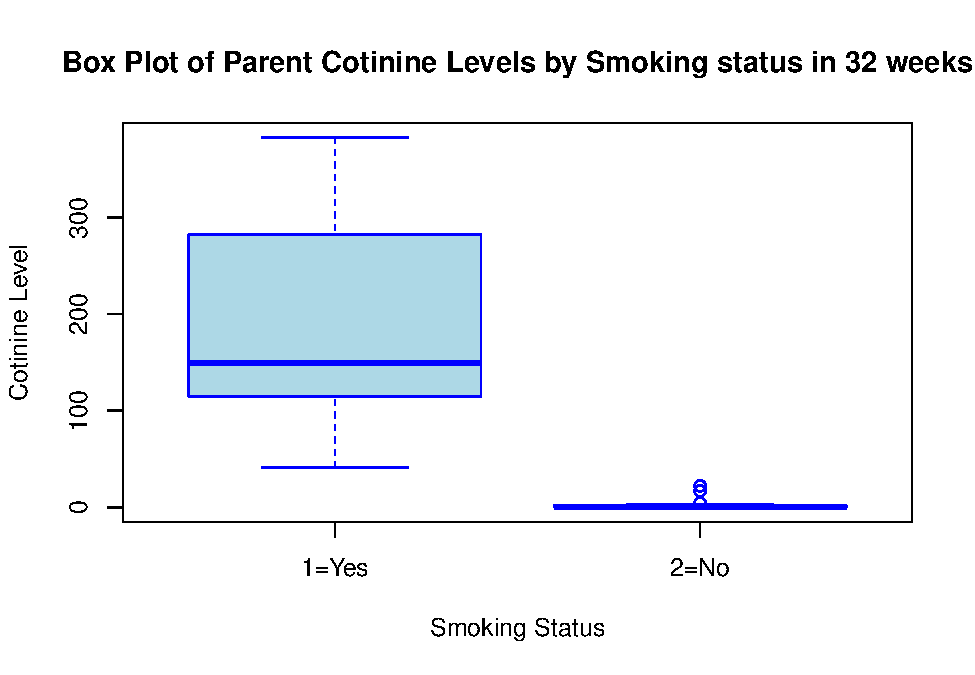
\includegraphics{Project-1-PHP-2550_files/figure-latex/unnamed-chunk-11-1.pdf}

\begin{Shaded}
\begin{Highlighting}[]
\CommentTok{\# Ensure \textquotesingle{}mom\_smoke\_16wk\textquotesingle{} column is a factor with a level for missing values}
\CommentTok{\# Create the summary table}

\NormalTok{tbl1\_swan}\OtherTok{\textless{}{-}}\NormalTok{ new\_df[,}\FunctionTok{c}\NormalTok{(}\DecValTok{32}\NormalTok{,}\DecValTok{33}\NormalTok{,}\DecValTok{81}\NormalTok{)] }\SpecialCharTok{\%\textgreater{}\%}
  \FunctionTok{tbl\_summary}\NormalTok{(}\AttributeTok{by =}\NormalTok{ cum\_smoke\_preg) }\SpecialCharTok{\%\textgreater{}\%}
  \FunctionTok{add\_p}\NormalTok{() }\SpecialCharTok{\%\textgreater{}\%}
  \FunctionTok{sort\_p}\NormalTok{() }\SpecialCharTok{\%\textgreater{}\%}
  \FunctionTok{modify\_caption}\NormalTok{(}\StringTok{"Compare Externalizing factor score with SDP in"}\NormalTok{) }
\FunctionTok{as\_kable\_extra}\NormalTok{(tbl1\_swan)}\SpecialCharTok{\%\textgreater{}\%} 
  \FunctionTok{kable\_styling}\NormalTok{(}\AttributeTok{full\_width=}\NormalTok{T, }\AttributeTok{latex\_options =} \FunctionTok{c}\NormalTok{(}\StringTok{\textquotesingle{}HOLD\_position\textquotesingle{}}\NormalTok{))}
\end{Highlighting}
\end{Shaded}

\begin{table}[H]

\caption{\label{tab:unnamed-chunk-12}Compare Externalizing factor score with SDP in}
\centering
\begin{tabu} to \linewidth {>{\raggedright}X>{\centering}X>{\centering}X>{\centering}X>{\centering}X>{\centering}X}
\hline
\textbf{Characteristic} & \textbf{0}, N = 34 & \textbf{1}, N = 3 & \textbf{2}, N = 1 & \textbf{3}, N = 10 & \textbf{p-value}\\
\hline
swan\_hyperactive & 4 (0, 7) & 12 (9, 13) & 0 (0, 0) & 10 (3, 18) & 0.11\\
\hline
swan\_inattentive & 8 (4, 12) & 10 (10, 11) & 0 (0, 0) & 14 (3, 17) & 0.3\\
\hline
\multicolumn{6}{l}{\rule{0pt}{1em}\textsuperscript{1} Median (IQR)}\\
\multicolumn{6}{l}{\rule{0pt}{1em}\textsuperscript{2} Kruskal-Wallis rank sum test}\\
\end{tabu}
\end{table}

\begin{Shaded}
\begin{Highlighting}[]
\NormalTok{tbl1\_bpm}\OtherTok{\textless{}{-}}\NormalTok{ new\_df[,}\FunctionTok{c}\NormalTok{(}\DecValTok{34}\NormalTok{,}\DecValTok{35}\NormalTok{,}\DecValTok{36}\NormalTok{,}\DecValTok{81}\NormalTok{)] }\SpecialCharTok{\%\textgreater{}\%}
  \FunctionTok{tbl\_summary}\NormalTok{(}\AttributeTok{by =}\NormalTok{ cum\_smoke\_preg) }\SpecialCharTok{\%\textgreater{}\%}
  \FunctionTok{add\_p}\NormalTok{() }\SpecialCharTok{\%\textgreater{}\%}
  \FunctionTok{sort\_p}\NormalTok{() }\SpecialCharTok{\%\textgreater{}\%}
  \FunctionTok{modify\_caption}\NormalTok{(}\StringTok{"Compare Externalizing factor score with SDP"}\NormalTok{) }
\FunctionTok{as\_kable\_extra}\NormalTok{(tbl1\_bpm)}\SpecialCharTok{\%\textgreater{}\%} 
  \FunctionTok{kable\_styling}\NormalTok{(}\AttributeTok{full\_width=}\NormalTok{T, }\AttributeTok{latex\_options =} \FunctionTok{c}\NormalTok{(}\StringTok{\textquotesingle{}HOLD\_position\textquotesingle{}}\NormalTok{))}
\end{Highlighting}
\end{Shaded}

\begin{table}[H]

\caption{\label{tab:unnamed-chunk-12}Compare Externalizing factor score with SDP}
\centering
\begin{tabu} to \linewidth {>{\raggedright}X>{\centering}X>{\centering}X>{\centering}X>{\centering}X>{\centering}X}
\hline
\textbf{Characteristic} & \textbf{0}, N = 34 & \textbf{1}, N = 3 & \textbf{2}, N = 1 & \textbf{3}, N = 10 & \textbf{p-value}\\
\hline
bpm\_int\_p & 1 (0, 3) & 2 (1, 2) & NA (NA, NA) & 3 (1, 5) & 0.2\\
\hline
\hspace{1em}Unknown & 6 & 0 & 1 & 2 & \\
\hline
bpm\_att\_p &  &  &  &  & 0.3\\
\hline
\hspace{1em}0 & 8 (32\%) & 1 (33\%) & 0 (NA\%) & 0 (0\%) & \\
\hline
\hspace{1em}1 & 7 (28\%) & 1 (33\%) & 0 (NA\%) & 3 (38\%) & \\
\hline
\hspace{1em}2 & 5 (20\%) & 1 (33\%) & 0 (NA\%) & 1 (13\%) & \\
\hline
\hspace{1em}3 & 1 (4.0\%) & 0 (0\%) & 0 (NA\%) & 0 (0\%) & \\
\hline
\hspace{1em}4 & 1 (4.0\%) & 0 (0\%) & 0 (NA\%) & 0 (0\%) & \\
\hline
\hspace{1em}5 & 2 (8.0\%) & 0 (0\%) & 0 (NA\%) & 1 (13\%) & \\
\hline
\hspace{1em}6 & 0 (0\%) & 0 (0\%) & 0 (NA\%) & 2 (25\%) & \\
\hline
\hspace{1em}7 & 1 (4.0\%) & 0 (0\%) & 0 (NA\%) & 0 (0\%) & \\
\hline
\hspace{1em}8 & 0 (0\%) & 0 (0\%) & 0 (NA\%) & 1 (13\%) & \\
\hline
\hspace{1em}Unknown & 9 & 0 & 1 & 2 & \\
\hline
bpm\_ext\_p &  &  &  &  & 0.7\\
\hline
\hspace{1em}0 & 13 (50\%) & 2 (67\%) & 0 (NA\%) & 3 (38\%) & \\
\hline
\hspace{1em}1 & 4 (15\%) & 1 (33\%) & 0 (NA\%) & 0 (0\%) & \\
\hline
\hspace{1em}2 & 4 (15\%) & 0 (0\%) & 0 (NA\%) & 1 (13\%) & \\
\hline
\hspace{1em}3 & 2 (7.7\%) & 0 (0\%) & 0 (NA\%) & 1 (13\%) & \\
\hline
\hspace{1em}4 & 1 (3.8\%) & 0 (0\%) & 0 (NA\%) & 1 (13\%) & \\
\hline
\hspace{1em}5 & 0 (0\%) & 0 (0\%) & 0 (NA\%) & 1 (13\%) & \\
\hline
\hspace{1em}7 & 1 (3.8\%) & 0 (0\%) & 0 (NA\%) & 1 (13\%) & \\
\hline
\hspace{1em}11 & 1 (3.8\%) & 0 (0\%) & 0 (NA\%) & 0 (0\%) & \\
\hline
\hspace{1em}Unknown & 8 & 0 & 1 & 2 & \\
\hline
\multicolumn{6}{l}{\rule{0pt}{1em}\textsuperscript{1} n (\%); Median (IQR)}\\
\multicolumn{6}{l}{\rule{0pt}{1em}\textsuperscript{2} Fisher's exact test; Kruskal-Wallis rank sum test}\\
\end{tabu}
\end{table}

\begin{Shaded}
\begin{Highlighting}[]
\CommentTok{\#Mean of bpm }
\NormalTok{tbl1\_bpm\_mean}\OtherTok{\textless{}{-}}\NormalTok{ new\_df[,}\FunctionTok{c}\NormalTok{(}\DecValTok{34}\SpecialCharTok{:}\DecValTok{36}\NormalTok{,}\DecValTok{81}\NormalTok{)] }\SpecialCharTok{\%\textgreater{}\%}
  \FunctionTok{tbl\_summary}\NormalTok{(}\AttributeTok{by =}\NormalTok{ cum\_smoke\_preg) }\SpecialCharTok{\%\textgreater{}\%}
  \FunctionTok{add\_p}\NormalTok{() }\SpecialCharTok{\%\textgreater{}\%}
  \FunctionTok{sort\_p}\NormalTok{() }\SpecialCharTok{\%\textgreater{}\%}
  \FunctionTok{modify\_caption}\NormalTok{(}\StringTok{"Compare Externalizing factor score with SDP"}\NormalTok{) }
\FunctionTok{as\_kable\_extra}\NormalTok{(tbl1\_bpm\_mean)}\SpecialCharTok{\%\textgreater{}\%} 
  \FunctionTok{kable\_styling}\NormalTok{(}\AttributeTok{full\_width=}\NormalTok{T, }\AttributeTok{latex\_options =} \FunctionTok{c}\NormalTok{(}\StringTok{\textquotesingle{}HOLD\_position\textquotesingle{}}\NormalTok{))}
\end{Highlighting}
\end{Shaded}

\begin{table}[H]

\caption{\label{tab:unnamed-chunk-12}Compare Externalizing factor score with SDP}
\centering
\begin{tabu} to \linewidth {>{\raggedright}X>{\centering}X>{\centering}X>{\centering}X>{\centering}X>{\centering}X}
\hline
\textbf{Characteristic} & \textbf{0}, N = 34 & \textbf{1}, N = 3 & \textbf{2}, N = 1 & \textbf{3}, N = 10 & \textbf{p-value}\\
\hline
bpm\_int\_p & 1 (0, 3) & 2 (1, 2) & NA (NA, NA) & 3 (1, 5) & 0.2\\
\hline
\hspace{1em}Unknown & 6 & 0 & 1 & 2 & \\
\hline
bpm\_att\_p &  &  &  &  & 0.3\\
\hline
\hspace{1em}0 & 8 (32\%) & 1 (33\%) & 0 (NA\%) & 0 (0\%) & \\
\hline
\hspace{1em}1 & 7 (28\%) & 1 (33\%) & 0 (NA\%) & 3 (38\%) & \\
\hline
\hspace{1em}2 & 5 (20\%) & 1 (33\%) & 0 (NA\%) & 1 (13\%) & \\
\hline
\hspace{1em}3 & 1 (4.0\%) & 0 (0\%) & 0 (NA\%) & 0 (0\%) & \\
\hline
\hspace{1em}4 & 1 (4.0\%) & 0 (0\%) & 0 (NA\%) & 0 (0\%) & \\
\hline
\hspace{1em}5 & 2 (8.0\%) & 0 (0\%) & 0 (NA\%) & 1 (13\%) & \\
\hline
\hspace{1em}6 & 0 (0\%) & 0 (0\%) & 0 (NA\%) & 2 (25\%) & \\
\hline
\hspace{1em}7 & 1 (4.0\%) & 0 (0\%) & 0 (NA\%) & 0 (0\%) & \\
\hline
\hspace{1em}8 & 0 (0\%) & 0 (0\%) & 0 (NA\%) & 1 (13\%) & \\
\hline
\hspace{1em}Unknown & 9 & 0 & 1 & 2 & \\
\hline
bpm\_ext\_p &  &  &  &  & 0.7\\
\hline
\hspace{1em}0 & 13 (50\%) & 2 (67\%) & 0 (NA\%) & 3 (38\%) & \\
\hline
\hspace{1em}1 & 4 (15\%) & 1 (33\%) & 0 (NA\%) & 0 (0\%) & \\
\hline
\hspace{1em}2 & 4 (15\%) & 0 (0\%) & 0 (NA\%) & 1 (13\%) & \\
\hline
\hspace{1em}3 & 2 (7.7\%) & 0 (0\%) & 0 (NA\%) & 1 (13\%) & \\
\hline
\hspace{1em}4 & 1 (3.8\%) & 0 (0\%) & 0 (NA\%) & 1 (13\%) & \\
\hline
\hspace{1em}5 & 0 (0\%) & 0 (0\%) & 0 (NA\%) & 1 (13\%) & \\
\hline
\hspace{1em}7 & 1 (3.8\%) & 0 (0\%) & 0 (NA\%) & 1 (13\%) & \\
\hline
\hspace{1em}11 & 1 (3.8\%) & 0 (0\%) & 0 (NA\%) & 0 (0\%) & \\
\hline
\hspace{1em}Unknown & 8 & 0 & 1 & 2 & \\
\hline
\multicolumn{6}{l}{\rule{0pt}{1em}\textsuperscript{1} n (\%); Median (IQR)}\\
\multicolumn{6}{l}{\rule{0pt}{1em}\textsuperscript{2} Fisher's exact test; Kruskal-Wallis rank sum test}\\
\end{tabu}
\end{table}

AIM 2: Explore links between self-regulation at baseline and substance
and externalizing at 6- and 12-month follow-ups.

AIM3: Identify self-regulation problems that mediate the link between
SDP/ETS exposure and level of, and change in, SU and EXT severity over
time.

\end{document}
